\documentclass[12pt,-letter paper]{article}
\usepackage{siunitx}              
\usepackage{setspace}
\usepackage{gensymb}
\usepackage{xcolor}
\usepackage{caption}
%\usepackage{subcaption}\doublespacing\singlespacing\usepackage[none]{hyphenat}
\usepackage{amssymb}
\usepackage{relsize}
\usepackage[cmex10]{amsmath}
\usepackage{mathtools}
\usepackage{amsmath}
\usepackage{commath}
\usepackage{amsthm}\interdisplaylinepenalty=2500
%\savesymbol{iint}
\usepackage{txfonts}%\restoresymbol{TXF}{iint}
\usepackage{wasysym}
\usepackage{amsthm}
\usepackage{mathrsfs}                                             
\usepackage{txfonts}
\let\vec\mathbf{}
\usepackage{stfloats}
\usepackage{float}
\usepackage{cite}
\usepackage{cases}
\usepackage{subfig}
%\usepackage{xtab}
\usepackage{longtable}
\usepackage{multirow}
%\usepackage{algorikage{amssymb}
%\usepackage{algpseudocode}
\usepackage{enumitem}
\usepackage{mathtools}
%\usepackage{eenrc}
%\usepackage[framemethod=tikz]{mdframed}                          
\usepackage{listings}                                             
%\usepackage{listings}
\usepackage[latin1]{inputenc}
%%\usepackage{color}{
%%\usepackage{lscape}
\usepackage{textcomp}
\usepackage{titling}
\usepackage{hyperref}
%\usepackage{fulbigskip}
\usepackage{tikz}
\usepackage{graphicx}
\lstset{frame=single,breaklines=true}
\let\vec\mathbf{}
\usepackage{enumitem}           
\usepackage{graphicx}            
\usepackage{siunitx}
\let\vec\mathbf{}
\usepackage{enumitem}
\usepackage{graphicx}
\usepackage{enumitem}
\usepackage{tfrupee}
\usepackage{amsmath}
\usepackage{amssymb}
\usepackage{mwe} % for blindtext and example-image-a in example
\usepackage{wrapfig}
\usepackage{amsmath}
\usepackage{graphicx}

\title{Probability}
\date{Dec 2023}
\begin{document}
\maketitle
\begin{enumerate}

\item A fair dice is thrown two times. Find the probability distribution of the number of sixes . Also determine the number of sixes.

\item A card from a pack of $52$ cards is lost. From the remaining cards of the pack, two cards are drawn randomly one-by-one without replacement and are found to be both kings. Find the probability of the lost card bring a king.

\item If the probability of an $E$ happening is $0.023$, then $P(\overline{E})$

\item Read the following passage and answer the questions given at the end:\\
\textbf{Diwali Fair}\\
A game in a booth at a Diwali Fair involves using a spinner first. Then if the spinner stops onan ever number, the player is allowed to pick a marble from a bag. The spinner and the marbles in the bag re represented in \figref{}fig:Probability.jpg}.
Prizes are given, when a black marble is picked. Shweta plays the game ones.

		\begin{figure}[H]
			\centering
			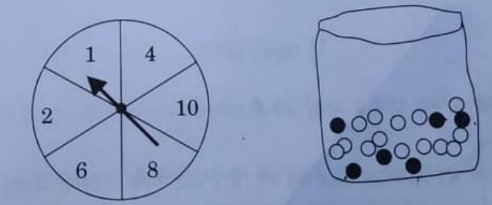
\includegraphics[width=0.5\columnwidth]{figs/Probability.jpg}
			\caption{A bag contains od marbles}
                        \label{fig:Probability.jpg}
		\end{figure}
\begin{enumerate}
\item What is the probability that she will be allowed to pick a marble from the bag?

\item Suppose she is allowed to pick a marble from the bag, what is the probability of getting a prize, when it is given that the contains $20$ balls out of which $6$ are black ?
\end{enumerate}
\end{enumerate}
\end{document}
